\documentclass[svgnames]{beamer}
%%\documentclass[svgnames,handout]{beamer}

%\usepackage[utf8]{inputenc}
\usepackage[T1]{fontenc}
\usepackage{graphicx}
\usepackage{longtable}
\usepackage{wrapfig}
\usepackage{rotating}
\usepackage[normalem]{ulem}
\usepackage{amsmath}
\usepackage{amssymb}
\usepackage{capt-of}
%\usepackage{hyperref}
\mode<beamer>{\usetheme{Berlin}}
\usecolortheme {spruce}

\usepackage[x11names]{xcolor}
\definecolor{Dark_Green}{rgb}{7, 74, 26}
\setbeamercolor{block title}{bg=DarkGreen, fg=white}
\setbeamercolor*{enumerate item}{fg=DarkGreen}
\setbeamercolor{itemize item}{fg=DarkGreen}
\setbeamercolor{itemize subitem}{fg=DarkGreen}
\setbeamercolor{enumerate item}{fg=DarkGreen}
\setbeamercolor{enumerate subitem}{fg=DarkGreen}
\setbeamercolor{enumerate subsubitem}{fg=DarkGreen}
%%--------------------------------------------------------------------------------
%%\usepackage[svgnames]{xcolor}
\usepackage{mathrsfs}
\usepackage{tikz-cd}

\usepackage{fontspec}
\setmonofont{FreeMono}
\setmainfont{FreeSerif}

\usepackage{unicode-math}

\usepackage[dvipsnames]{xcolor}

\usepackage{amsthm}
\usepackage{thmtools}
%\usepackage{cleveref}

%\usepackage[cachedir=mintedcache]{minted}
\usepackage{minted}
\usemintedstyle{tango}
\setminted[bash]{bgcolor=NavajoWhite}
\setminted[output]{bgcolor=NavajoWhite}
\setminted[python]{bgcolor=Lavender}

\newmintinline[lean]{lean4}{bgcolor=lavender}
\newminted[leancode]{lean4}{fontsize=\footnotesize,bgcolor=Lavender}
\setminted[lean]{bgcolor=LightBlue}

\usepackage{newunicodechar}
\newfontfamily{\freeserif}{DejaVu Sans}
\newunicodechar{✝}{\freeserif{✝}}
\newunicodechar{∀}{\ensuremath{\forall}}
\newunicodechar{→}{\ensuremath{\to}}
\newunicodechar{≤}{\ensuremath{\le}}
\newunicodechar{⧸}{/}


\newcommand{\Z}{\mathbf{Z}}
\newcommand{\Q}{\mathbf{Q}}
\newcommand{\R}{\mathbf{R}}
\newcommand{\C}{\mathbf{C}}
\newcommand{\F}{\mathbf{F}}
\newcommand{\N}{\mathbf{N}}

\newcommand{\LL}{\mathscr{L}}
\newcommand{\pp}{\mathbf{p}}
\newcommand{\xx}{\mathbf{x}}
\newcommand{\yy}{\mathbf{y}}
\newcommand{\vv}{\mathbf{v}}
\newcommand{\ww}{\mathbf{w}}
%%--------------------------------------------------------------------------------
\author{Clea Bergsman, Katherine Buesing, Sahan Wijetunga}
\date{2025-07-10}
\title{Formalization and Finite Algebra}
\hypersetup{
 pdfauthor={Clea Bergsman, Katherine Buesing, Sahan Wijetunga},
 pdftitle={Formalization and Finite Algebra},
 pdfkeywords={modelling},
 pdfsubject={},
 pdfcreator={Emacs 31.0.50 (Org mode 9.7.11)}, 
 pdflang={English}}
\usepackage{biblatex}

\begin{document}
\section{Introduction}
% table of contents slide 
\maketitle
\begin{frame}{Outline}
\tableofcontents
\end{frame}

%Clea
\section {Nondegenerate Bilinear Forms}
\subsection{Definitions}

\setbeamertemplate{blocks}[rounded][shadow=true]

\begin{frame}{Recall: What is a Bilinear Form?}
\begin{block}{Definition}
A \textbf {bilinear form} is a map $\beta : V\times W \to K $, where V and W are K-vector spaces and K is a field, when
\begin{itemize}
    \item $\beta (v_1 + v_2 , w) = \beta (v_1 , w) +\beta ( v_2,w)$
    \item $\beta ( v, w_1 + w_2) = \beta (v,w_1) +\beta (v , w_2)$
    \item $\beta(\lambda v, w) = \beta (v, \lambda w) = \lambda \beta (v , w)$
\end{itemize}
hold for all $v\in V$, $w\in W$, and $\lambda \in K$.
\end{block}
\end{frame}

\begin{frame}{Recall: Symmetric, Alternating, and Skew Bilinear Forms}

\begin{block}{Symmetric}
$\beta (v,w) = \beta (w,v)$ $\forall$ $v,w$
\end{block}

\begin{block}{Alternating}
$\beta (v,v) = 0$, $\forall$ $v$
\end{block}

\begin{block}{Skew}
$\beta (v,w) = -\beta (w,v)$, $\forall$ $v,w$
\end{block}

Note: Bilinear forms that are \textbf{anti-symmetric} are both alternating and skew-symmetric.
\end{frame}

\subsection{Reflexive Proofs}
\begin{frame}{Reflexive Bilinear Forms}
\begin{block}{Definition}
A bilinear form $\beta$ is \textbf{reflexive} if
$\beta(v,w)=0\iff\beta(w,v)=0$ $\forall$ $v,w\in V$
\end{block}
\end{frame}

{\tiny
\begin{minted}[]{lean}
lemma alt_is_reflexive (β:BilinForm k V) (h:Alt β) : IsRefl β := by
  intro v w l
  have hv : β v v = 0 := by apply h
  have hw : β w w = 0 := by apply h
  have h1 : β (v+w) (v+w) = (β v) v + (β w) v + (β v) w + (β w) w :=
    calc
    (β (v+w)) (v+w) = (β v) (v+w) + (β w) (v+w) := by 
        rw [LinearMap.BilinForm.add_left]
    _ = (β v) v + (β w) v + (β v) w + (β w) w := by
      rw [LinearMap.BilinForm.add_right v v w, LinearMap.BilinForm.add_right w v w, 
        ← add_assoc]; ring
  have hvw : β (v+w) (v+w) = 0 := by apply h
  rw [hv, hw, hvw, zero_add, add_zero, add_comm] at h1
  have h2: 0 + -(β w) v = (β v) w + (β w) v + -(β w) v := by
    apply (@add_right_cancel_iff _ _ _ (-(β w) v) 0 ((β v) w + (β w) v)).mpr h1
  rw [l, zero_add] at h1
  symm at h1
  exact h1
\end{minted}
}

{\tiny
\begin{minted}[]{lean}
lemma symm_is_reflexive (β:BilinForm k V) (h:Symm β) : 
    IsRefl β := by
  intro v w l
  have h1: (β v) w = (β w) v := by apply h
  rw [l] at h1
  symm at h1
  exact h1
\end{minted}
}

\subsection{Matrices}
\begin{frame}{Bilinear Forms as Matrices}
\begin{itemize}[<+->]
    \item % Bilinear Form as matrix  
    Given a basis $(v_1, \dots, v_n)$ for $V$ we can form a matrix $A$ corresponding to the bilinear form $B: V \times V \to k$ by defining $A_{ij} := B(v_i, v_j)$. Thus,
    \[B(x,y) = [x]^TA[y]\]
    for $x,y \in V$. 
    \item The dot product on $\R^n$ has matrix \[
I_n = \begin{bmatrix}
1 & 0 & \cdots & 0 \\
0 & 1 & \cdots & 0 \\
\vdots & \vdots & \ddots & \vdots \\
0 & 0 & \cdots & 1
\end{bmatrix}
\]
\end{itemize}
\end{frame}
\begin{frame}{Bilinear Forms as Matrices}
\begin{itemize}[<+->]
    \item Symmetric forms have matrix satisfying $A^T=A$. 
       \[
    \begin{bmatrix}
    1 & 2 \\
    2 & 3
    \end{bmatrix}
    \]
    \item Alternating forms have matrix satisfying $A^T=-A$. 
        \[
    \begin{bmatrix}
    0 & 5 \\
    -5 & 0
    \end{bmatrix}
    \]
    \item Nondegenerate forms have matrix with $\det(A)\neq 0$. 
        \[
    \begin{bmatrix}
    1 & 2 \\
    3 & 4
    \end{bmatrix}
    \quad (\det = 4\cdot 1-3 \cdot 2\neq 0)
    \]
\end{itemize}
\end{frame}

\subsection{Nondegenerate Proofs}
\begin{frame}{Nondegenerate Definition}
\begin{Theorem}
Let $\beta$ be a bilinear form on $V$, $M=[\beta(v_i,v_j)]$, and $v_1, . . . , v_n$ a basis of $V$
The following are equivalent:
\begin{itemize}
    \item $det(M) \neq 0$
    \item $\forall w \in V $ $\beta (v,w) = 0 \implies v=0$
    \item $\forall v \in V $ $\beta (v,w) = 0 \implies w=0$
\end{itemize}
\end{Theorem}
\end{frame}

{\scriptsize
\begin{minted}[]{lean}
theorem nondeg_rank (β : BilinForm k V) [FiniteDimensional k V] 
(n : ℕ ) (h: Module.rank k V = n) (b : Basis (Fin n) k V): 
  (LinearMap.BilinForm.Nondegenerate β) ↔ 
  Matrix.rank (BilinForm.toMatrix b β ) = n := by
  constructor
  -- Nondegenerate β → rank M = n
  intro hn
  have nondeg : β.Nondegenerate := by apply hn
  have nul_zero : LinearMap.ker β = ⊥ := by
    apply LinearMap.BilinForm.nondegenerate_iff_ker_eq_bot.mp; 
    exact nondeg
  let M : Matrix (Fin n) (Fin n) k := BilinForm.toMatrix b β
  have h1 : Module.rank k ↥(range β ) + (Module.rank k (ker β)) 
  = Module.rank k V  :=
      by apply LinearMap.rank_range_add_rank_ker
  have zero : (Module.rank k ↥(ker β)) = 0 := by 
  rw [nul_zero]; simp
  rw [zero, add_zero] at h1
  rw [h] at h1
  simp at h1
  exact h1
  \end{minted}
  
  \begin{minted}[]{lean}
  --  rank M = n → Nondegenerate β
  intro hn
  have h1 : Module.rank k ↥(range β ) + (Module.rank k (ker β)) 
  = Module.rank k V  :=
      by apply LinearMap.rank_range_add_rank_ker
  simp at h1
  rw [hn] at h1
  have nul_zero : Module.rank k ↥(ker β) = 0 := by
    apply (add_eq_left _ _ (↑n) (Module.rank k ↥(ker β))).mp
    at h1
  simp at nul_zero
  apply LinearMap.BilinForm.nondegenerate_iff_ker_eq_bot.mpr
  exact nul_zero
\end{minted}
}

% katherine 
\section{Pen and Paper vs. Lean}
\label{sec:"proof-comparison"}

\subsection{Theorems}

\begin{frame}[label={sec:proof_comparison}]{Creating a Basis using Disjoint Bases}
% \begin{itemize}[<+->]
\begin{Theorem}
Let $V$ be a vector space over a field $k$, and let $W_1$ and $W_2$ be subspaces of $V$ such that $W_1 + W_2 = V$ and $W_1 \cap W_2 = \{0\}$. Let $B_1$ and $B_2$ be bases of $W_1$ and $W_2$, respectively. 
\begin{itemize}
    \item We can create a basis for $V$ using the union of $B_1$ and $B_2$
\end{itemize}
\end{Theorem}


\end{frame}

\begin{frame}[label={sec:proof_comparison}]{Additional Theorems}

\begin{Theorem}
Let $V$ be a vector space over a field $k$, and let $W_1$ and $W_2$ be subspaces of $V$ such that $W_1 \cap W_2 = \{0\}$. Let $e_1$ and $e_2$ be linearly independent sets of $W_1$ and $W_2$, respectively. 
\begin{itemize}
    \item The disjoint union of $e_1$ and $e_2$ is linearly independent.
\end{itemize}
\end{Theorem}

\begin{Theorem}
Let $V$ be a vector space over a field $k$, and let $W_1$ and $W_2$ be two subspaces of a larger vector space $V$, where the direct sum of $W_1$ and $W_2$ is equal to $V$. Let $s_1$ and $s_2$ be sets of vectors that span $W_1$ and $W_2$, respectively.
\begin{itemize}
    \item The union of $s_1$ and $s_2$ span $V$. 
\end{itemize}
\end{Theorem}

\end{frame}

\begin{frame}[label={sec:proof_comparison},fragile]{Additional Theorems in Lean}
\begin{itemize}
\item Theorem: Linear independence by transverse subspaces

{\scriptsize
\begin{minted}[]{lean}
theorem lin_indep_by_transverse_subspaces
   (k V : Type) [Field k] [AddCommGroup V] [Module k V] 
   (I₁ I₂ : Type) [Fintype I₁] [Fintype I₂]
   (b₁ : I₁ → V) (b₂ : I₂ → V)
   (b1_indep : LinearIndependent k b₁)
   (b2_indep : LinearIndependent k b₂)
   (W₁ W₂ : Submodule k V) (h_int : W₁ ⊓ W₂ = ⊥)
   (hbw1 : ∀ i, b₁ i ∈ W₁) (hbw2 : ∀ i, b₂ i ∈ W₂)
   [DecidableEq I₁] [DecidableEq I₂]
   : LinearIndependent k (Sum.elim b₁ b₂)
\end{minted}
}

\end{itemize}
\end{frame}

\begin{frame}[label={sec:proof_comparison},fragile]{Additional Theorems in Lean Continued}
\begin{itemize}
\item Theorem: Span of union of sets 

{\scriptsize
\begin{minted}[]{lean}
lemma union_span' (W₁ W₂ : Submodule k V) (s₁ s₂ : Set V)
  (hs₁: W₁ = Submodule.span k s₁)
  (hs₂: W₂ = Submodule.span k s₂)
  (hw: ⊤ = W₁ ⊔ W₂)
  : ⊤ = Submodule.span k (s₁ ∪ s₂)
\end{minted}
}

\end{itemize}
\end{frame}

\subsection{Proofs}
\begin{frame}[label={sec:proof_comparison}]{Pen and Paper Proof}
 \begin{itemize}[<+->]
\item In order to show that the disjoint union of bases $B_1$ and $B_2$ is a basis for $V$, we want to show that this disjoint union is both linearly independent and spans the entirety of V. 
\item Since $W_1 \cap W_2 = \{0\}$, and $B_1$ and $B_2$ are both individually linearly independent, we can conclude that their union is linearly independent.
\item Now we want to show that their union spans all of V. Since $W_1 + W_2 = V$, and $B_1$ and $B_2$ span $W_1$ and $W_2$, respectively, we can conclude that their union spans V. 
\end{itemize}
\end{frame}

\begin{frame}[label={sec_proof_comparison},fragile]{Lean Proof}

{\scriptsize
\begin{minted}[]{lean}
def basis_of_direct_sum
        (W₁ W₂ : Submodule k V)
        (ι₁ ι₂ : Type) [Fintype ι₁] 
        [Fintype ι₂]
        (B₁ : Basis ι₁ k W₁)
        (B₂ : Basis ι₂ k W₂)
        (hspan : W₁ ⊔ W₂ = (⊤: Submodule k V))
        (hindep : W₁ ⊓ W₂ = (⊥:Submodule k V))
        [DecidableEq ι₁] [DecidableEq ι₂] 
        [FiniteDimensional k V]:
        Basis (ι₁ ⊕ ι₂) k V := by
\end{minted}
}

\end{frame}

\begin{frame}[label={sec_proof_comparison},fragile]{Lean Proof}

{\scriptsize
\begin{minted}[]{lean}

have hli: LinearIndependent k (Sum.elim 
(W₁.subtype ∘ B₁) (W₂.subtype ∘ B₂)) := by
    apply lin_indep_by_transverse_subspaces
    · apply LinearIndependent.map' B₁.linearIndependent W₁.subtype 
    (by simp)
    · apply LinearIndependent.map' B₂.linearIndependent W₂.subtype 
    (by simp)
    · have k₀ : Disjoint W₁ W₂ := by
        rw[disjoint_iff]
        exact hindep
        rw[Disjoint.eq_bot k₀]
    · simp
    · simp
\end{minted}
}

\end{frame}

\begin{frame}[label={sec_proof_comparison},fragile]{Lean Proof}

{\scriptsize
\begin{minted}[]{lean}
 have hsp: ⊤ ≤ Submodule.span k (Set.range (Sum.elim 
 (W₁.subtype ∘ B₁) (W₂.subtype ∘ B₂))) := by
    simp
    rw[union_span'] 
    exact W₁
    exact W₂
    · exact span_range (Basis.span_eq B₁)
    · exact span_range (Basis.span_eq B₂)
    · rw[hspan]
    exact Basis.mk hli hsp
\end{minted}
}

\end{frame}
% katherine 



% \subsection{Section one}
% \label{sec:one}
% \begin{frame}[label={sec:examples},fragile]{Lean examples}
%  \begin{itemize}[<+->]
% \item example: defn of convergence of a sequence

% \begin{minted}[]{lean}
% -- definition of "u tends to ℓ" 
% def seq_limit (u : ℕ → ℝ) (ℓ : ℝ) :=
%   ∀ ε > 0, ∃ N, ∀ n ≥ N, |u n - ℓ| ≤ ε
% \end{minted}
% \end{itemize}
% \end{frame}

% \begin{frame}[label={sec:appending-lists},fragile]{appending lists}
%  \begin{itemize}[<+->]
% \item Here is some \texttt{Lean} code that \emph{appends two lists}.
% \begin{minted}[]{lean}
% def append {α:Type} (xs ys : List α )
%   : List a :=
%   match xs with
%   | [] => ys
%   | z :: zs => z :: append zs ys
% \end{minted}

% \item e.g.
% \begin{minted}[]{lean}
% append ["a", "b", "c"] ["d", "e"]
% \end{minted}
% evaluates to
% \begin{minted}[]{lean}
% ["a", "b", "c", "d", "e"] : List String
% \end{minted}
% \end{itemize}
% \end{frame}





% \begin{frame}[label={sec:vector-spaces}]{vector spaces}
% \begin{itemize}[<+->]
% \item Let \(k\) be a \alert{field}.

% \item and let \(V\) be a finite dimensional vector space over \(k\).

% \item Let \(\beta:V \times V \to k\) be a \alert{bilinear form}

% \item and suppose that \(\beta\) is \alert{nondegenerate} and \alert{symmetric}

% \item (also suppose for convenience that \(p\neq 2\) where \(p\) is the characteristic of \(k\))
% \end{itemize}
% \end{frame}

%Sahan
\section{Hyperbolic}


\begin{frame}{Hyperbolic Forms}
\small
% 2d-space hyperbolic defn
% generic hyperbolic defn
\begin{itemize}[<+->]
\item A 2-dimensional vector space $V$ is called \textbf{Hyperbolic} if there exists a basis $(e, f)$ such that the form has matrix 
\[H_2=\begin{pmatrix}
    0 & 1\\
    * & 0
\end{pmatrix}\]
\item Note if $V$ is symmetric as well, it has matrix $\begin{pmatrix}
    0 & 1\\
    1 & 0
\end{pmatrix}$, and if alternating then matrix $\begin{pmatrix}
    0 & 1\\
    -1 & 0
\end{pmatrix}$. 
\item A generic vector space $V$ is \textit{Hyperbolic} if it has a basis making its form equal to                $\begin{bmatrix}H_2 & &  &  \\ & H_2 &  &  \\ &  & \ddots &  \\ &  &  & H_2\end{bmatrix}$
\end{itemize}

\end{frame} 



\subsection{Alternating Forms}
\begin{frame}{Alternating is Hyperbolic}
\begin{block}{Theorem}
Every nondegenerate (finite dimensional) alternating bilinear form $B$ on $V$ is Hyperbolic. 
\end{block}
\end{frame}


\begin{frame}{Pen and Paper Proof {\tiny(That nondegenerate (finite dimensional) alternating bilinear forms are Hyperbolic)}}
\begin{itemize}[<+->]
\item If $V \neq 0$, pick $e \neq 0$ in $V$. 
\begin{itemize}
    \item From nondegeneracy, pick $v$ with $B(e,v)\neq 0$. 
    \item From scaling, pick $f=\lambda v$ with $B(e,f)=1$. 
\end{itemize}
\item Then $H=\text{Span}(e,f)$ has matrix $\begin{pmatrix}
    0 & 1 \\ -1 & 0
\end{pmatrix}$ and is Hyperbolic. 
\item Fact: $V = H \oplus H^\perp $. 
\item Check: 
\begin{itemize}
    \item $H^\perp$ Alternating
    \item $H^\perp$ Nondegenerate
    \item $\dim(H^\perp)<\dim(V)$
\end{itemize}
\item From induction, $H^\perp$ is Hyperbolic. 
\pause Thus, 
{\tiny \[A_V = \begin{pmatrix}
    A_H & 0\\
    0 & A_{H^\perp}
\end{pmatrix} = \begin{pmatrix}
    \begin{pmatrix}
    0 & 1 \\ -1 & 0
\end{pmatrix} & \\
& \begin{pmatrix}H_2 & &   \\   & \ddots &  \\ &   & H_2\end{pmatrix}
\end{pmatrix} = \begin{pmatrix}H_2 & &  &  \\ & H_2 &  &  \\ &  & \ddots &  \\ &  &  & H_2\end{pmatrix}
\]}
\end{itemize}
\end{frame}


\begin{frame}[label={sec_proof_comparison},fragile]{Lean Proof {\tiny(That nondegenerate (finite dimensional) alternating bilinear forms are Hyperbolic)}}

% 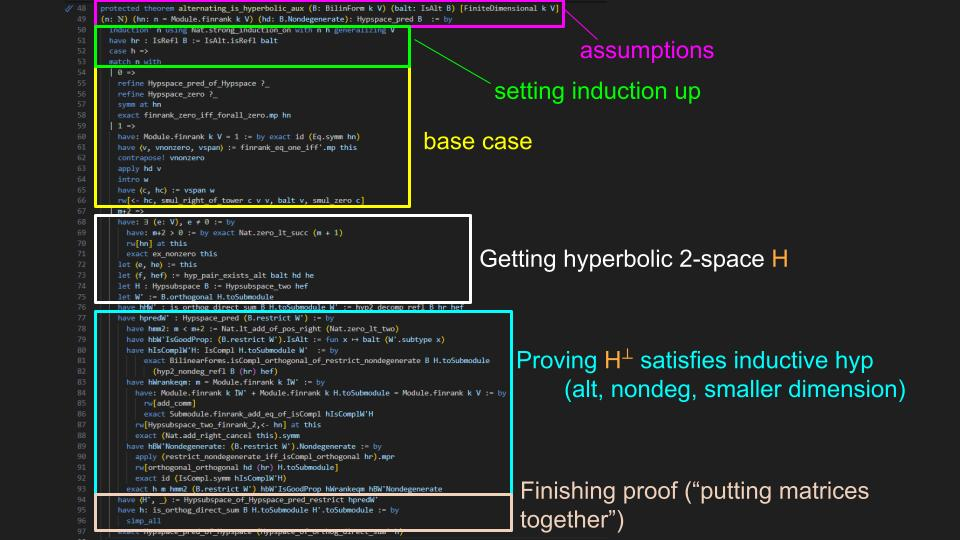
\includegraphics[width=1.0\linewidth]{lean proof alternating.jpg}
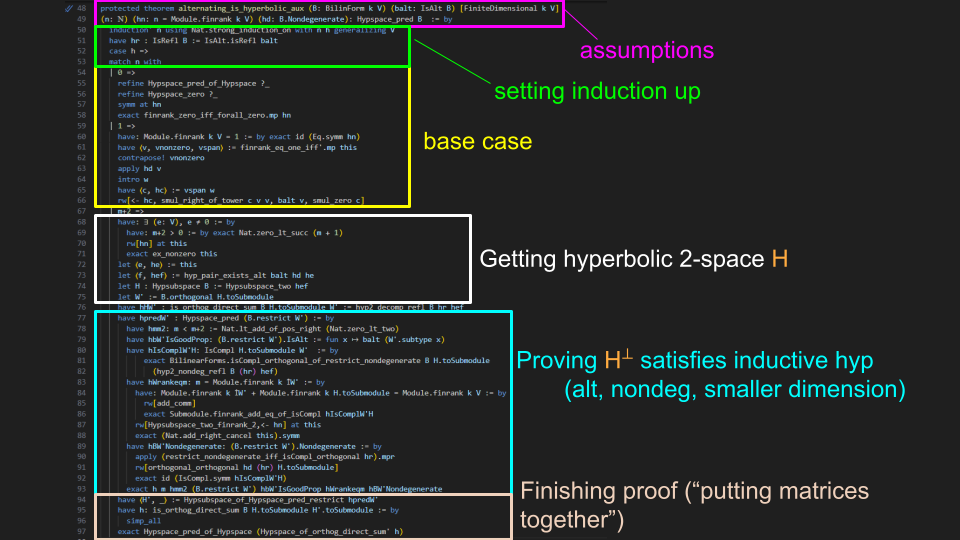
\includegraphics[width=1\linewidth]{lean alternating.png}
\end{frame}


\begin{frame}{Lean Proof v.s. Paper Proof}


The lean proof was
\pause
\begin{itemize}[<+->]
    \item Quick
    \item Efficient
    \item Similar in length and style to the paper one
    \item Relied heavily on the power of Mathlib and a >1000 line auxiliary file setting up the theory of Hyperbolic spaces
\end{itemize}
\end{frame}

\subsection{Symmetric Forms}
\begin{frame}{Symmetric Forms}
\begin{itemize}[<+->]
\begin{block}{Theorem}
Every nondegenerate (finite dimensional, field characteristic not $2$) symmetric bilinear form is the direct sum of a Hyperbolic form and a definite (anisotropic) form. 
\end{block}
\item The paper proof is similar in length to the alternating one. 
\item The lean proof was 10x longer
\begin{itemize}[<+->]
    \item Involves subspaces and ``direct sum''
\end{itemize}
\end{itemize}
\end{frame}

\begin{frame}[label={sec_proof_comparison},fragile]{Lean Hyperbolic Space Definitions}

{\scriptsize
\begin{minted}[]{lean}
@[ext]
structure Hypspace (B: BilinForm k V) where
  I: Type
  basis : Basis (I ⊕ I) k V
  pred: Hypspace_fun_pred B basis

...

@[ext]
structure Hypsubspace (B: BilinForm k V) where
  I: Type
  coe : I ⊕ I → V
  pred: Hypspace_fun_pred B coe
\end{minted}
}

\end{frame}


\section{Conclusion}

\begin{frame}{References}
\begin{enumerate}
\item Avigad, J. Buzzard, K. Lewis R. Y. Massot, P. (2020). \textit{Mathematics in Lean}. 
\item Liesen, J. Mehrmann, V. (2015). \textit{Linear Algebra}.
\item Reich, E. (2005, February 28). Bilinear Forms. Retrieved July 10, 2005, from https://math.mit.edu/~dav/bilinearforms.pdf

\end{enumerate}
\end{frame}


\begin{frame}
	    \begin{center}
	        \textbf{Thank you!}\\
	        
	        Special thanks to Dr. George McNinch and the REU
         \bigbreak
         \LARGE
       
	    \end{center}
\end{frame}



\end{document} 